\chapter{Detecting Linear Structure}





\section{Curvilinear Structure Detection and Orientation Estimation}

For the four learning methods (DT-CWT/RF, Monogenic/RF, Linop/RF, Gaussian/RF), we first constructed random forests to classify between structure and background pixels and to compute an estimate of orientation at each pixel.

All forests were constructed with 200 trees and following published guidelines~\cite{Breiman_ML01}. However, rather than using a single set of training data from which samples were drawn with replacement (\ie bootstrapping), we used our method for randomly generating unique synthetic lines images (as described in \ref{s:}) to construct a new training sample at each tree-building step. For detection, each sample comprised 100k curvilinear structure pixels and 100k background pixels, whilst for orientation regression we used 200k pixels all belonging to curvilinear structure. 

Thus for any given representation (DT-CWT, Monogenic, Linop, Gaussian) and forest (classification, regression) we applied the following scheme:

\begin{enumerate}
\item	Generate a new synthetic line image with known ground truth
\item Extract feature vectors for a random set of pixels in the image
\item Repeat 1 and 2 until training sample complete
\item Construct tree using the CART algorithm
\item Repeat 1 to 4 until 200 trees constructed
\end{enumerate}

Details on the composition of feature vectors for each representation type are given below. Note for all methods, the number of scales used $s$ and the neighbourhood size $w$ were empirically tested to select the best combination for each method. In each case, we tried $s$ = 3, 4, 5, 6 and $w$ = 1, 3. For reasons of space, results are shown only for the best combination in each method.

\begin{itemize}
\item	DT-CWT/RF: images were decomposed using the DT-CWT to s scales. Neighbourhoods of interpolated phase and magnitude coefficients were extracted in each of the 6 oriented subbands producing a feature vector of 12w2s elements.
\item	Monogenic/RF: the monogenic signal was extracted across s scales, with the initial wavelength set at $\lambda$ = 4 pixels. Neighbourhoods of phase, amplitude and orientation values were computed giving a total feature size of 3 w2s. 
\item	Linop/RF: 8 oriented line filters were computed at each scale. Collecting neighbourhoods of the oriented filter responses produced 8w2s elements in each feature vectors.
\item	Gaussian/RF: for the Gaussian 2nd derivative method, the three directional derivatives were applied to an image at each scale. The standard deviation of the smallest kernel was 1 pixel, subsequent kernels increased by a factor of 2 at each scale. As with Monogenic/RF this resulted in feature vectors with 3w2s elements.
\end{itemize}

For testing, feature vectors for each representation were extracted at all pixels in the 100 synthetic test images. The classification and regression forests were then used to compute a line detection score (the proportion of votes for the curvilinear structure class) and orientation (the mean output of each regression tree, with appropriate angular wrapping at 0\deg and 180\deg) at each pixel. Example results of line detection are shown in~\ref{f:synthetic_responses}.

In addition to the four learning methods, the prescriptive variants of the Monogenic, Linop and Gaussian approaches were applied to the test images, example results of which are depicted in \ref{f:synthetic_responses}.

ROC curves for the seven methods tested are shown in~\ref{f:} 2, using the known ground-truth for the test images to define pixels on the centrelines of curvilinear structures as foreground, and pixels lying outside the structures as background. Areas under the ROC curves and detection sensitivities at a fixed specificity of 90\% are shown in~\ref{t:}. For orientation, only pixels belonging to curvilinear structures (although not necessarily at the centerline) were included in the results. The absolute differences between the predicted and known orientations (with appropriate angle wrapping) were taken, and used to generate cumulative distribution functions of orientation errors for each method, as shown in~\ref{f:}. The mean absolute errors of the estimated orientations are also included in~\ref{t:}.

These results show that the four learning methods perform significantly better than the three prescriptive methods (with the exception of orientation computation in Monogenic/RF). DT-CWT/RF is significantly the strongest performing for both line detection and orientation estimation, followed by Linop/RF then Gaussian/RF.

As expected, because Linop, of the three prescriptive methods, discards the highest proportion of filter responses, Linop/RF gains the most from training. This highlights the ability of the random forests to extract useful information from a rich local description of image content, and whilst we do not have a prescriptive variant to compare it to, we believe this shows the importance of training in maximizing the benefit of using the DT-CWT. We also note that the added information that can be gained from the DT-CWT representation results from an increase in the richness of the local description of texture and is not due to increasing the support of the descriptor. Indeed, as described above we tested all representations over an equivalent range of filter scales so that the same image support was available to each method.

The orientation results for both Monogenic and Monogenic/RF were surprisingly poor. Counter-intuitively, visual analysis of the test outputs showed that the Monogenic methods performed particularly badly at the exact centerline of curvilinear structures, where an essentially random orientation appeared to be returned. This is in contrast to the other tested methods that, as expected, performed strongest along the centerlines of structures. Computing estimation errors at pixels belonging to structures but not lying on the centerline produces a small improvement in the results (mean absolute errors of 32.55\deg and 29.39\deg for the RF and prescriptive variant respectively), though even then performance lags behind the other tested methods and of course in a real image we do not know the precise location of structure centerlines. Determining why orientations are estimated so poorly by the monogenic signal at the centre of structures, where in theory the signal is strongest, may warrant further investigation.

To show qualitative results for real mammograms, the seven methods were applied to detect curvilinear structures and estimate orientation for the malignant regions described in section 5.1. Example detection results are shown in \ref{f:}. Assessing the results visually, it would appear that the outputs of the learning based methods (and particularly DT-CWT/RF, Linop/RF and Gaussian/RF) are similar to the output of synthetic data whilst capturing the key curvilinear structures in the real regions. This would suggest our model for producing synthetic lines generates good data from which to train random forests for real images. Of course validating this hypothesis is important and we are currently working on a quantitative evaluation of the methods in real data when used, for example, as part of a larger lesion detection scheme.

In terms of applying the learning methods to real images, it is worth noting how the methods scale with increasing image size - particularly above the point at which the set of feature vectors for all image pixels can be stored in working memory. For the DT-CWT, provided the initial decomposition can be stored in memory (which due to its low-redundant decimating construction is possible even for full size mammograms of the order 3000x2400 pixels) then interpolated coefficients can be efficiently sampled to generate feature vectors for block-wise regions of the image. Each block of feature vectors can be classified by the forest and cleared from working from memory storing only the output of the forest. In this way only a small overhead is introduced for block-wise classifying the image. However, for the other methods it becomes necessary to interleave the decomposition of the image with the sampling of feature vectors. For example, it may be necessary to apply the filters at a single scale, extract features for that scale for a particular block of the image, filter at the next scale and extract those features, and so on. Of course, when the complete feature vectors for a single block have been classified, the process repeats. Thus a large image may in fact end up by decomposed many times over introducing a large computational overhead for block-wise processing. The point at which this cost occurs will depend on the size of the image and the type of representation used. Obviously the cost is worst for Linop which requires storing 8 (\ie the number orientations) full copies of the image at each scale, compared to just 3 for the Gaussian and Monogenic methods.


\begin{figure}
\centering
\begin{tabular}{c c}
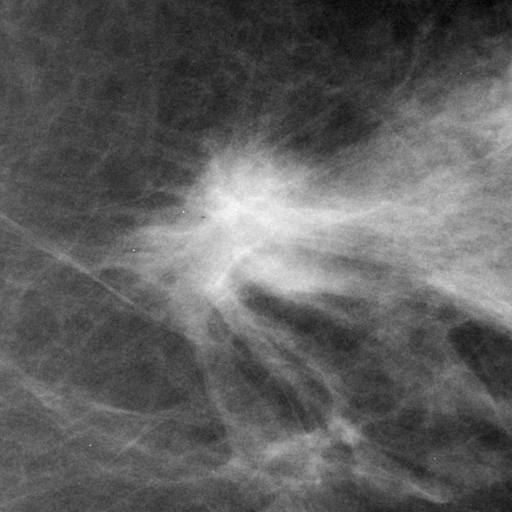
\includegraphics[width=\qtrcol]{\figpath/ipmi/mass046} &
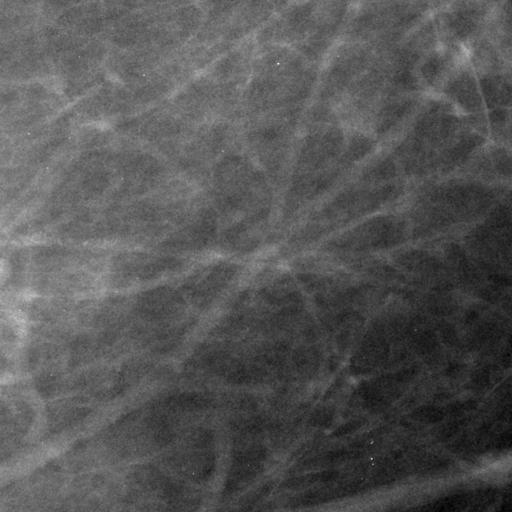
\includegraphics[width=\qtrcol]{\figpath/ipmi/norm068} \\
(a) & (b) \\
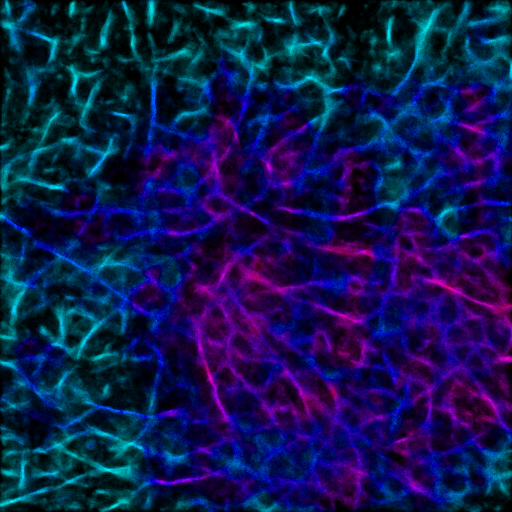
\includegraphics[width=\qtrcol]{\figpath/ipmi/spic_prob_mass046_a} &
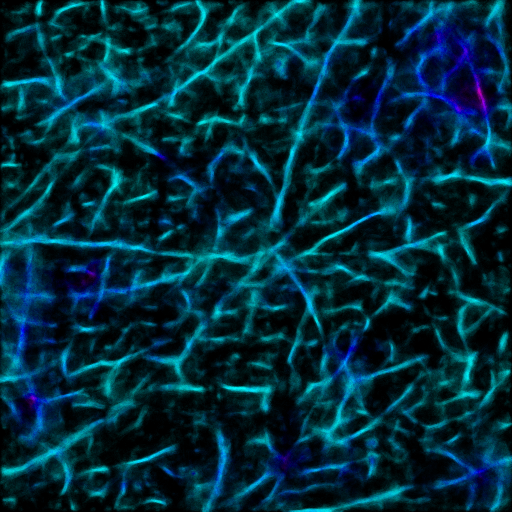
\includegraphics[width=\qtrcol]{\figpath/ipmi/spic_prob_norm068_a} \\
(c) & (d)
\end{tabular}
%
\caption{Regions depicting (a) malignant and (b) normal tissue. The corresponding spicule classification results are depicted in (c,d) using hue to indicate abnormality -- ranging from cyan (normal) to pink (spicule) -- and intensity to indicate the line detection output from the DT-CWT method.}
\label{f:mammogram_examples}
\end{figure}


\begin{figure}
\centering
\begin{tabular}{c c c c}
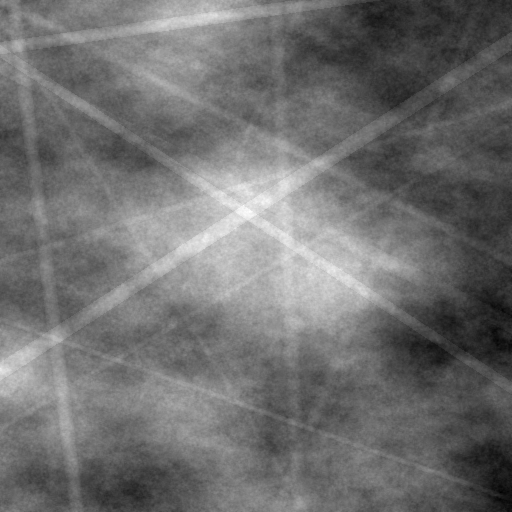
\includegraphics[width=\qtrcol]{\figpath/ipmi/line512_003} &
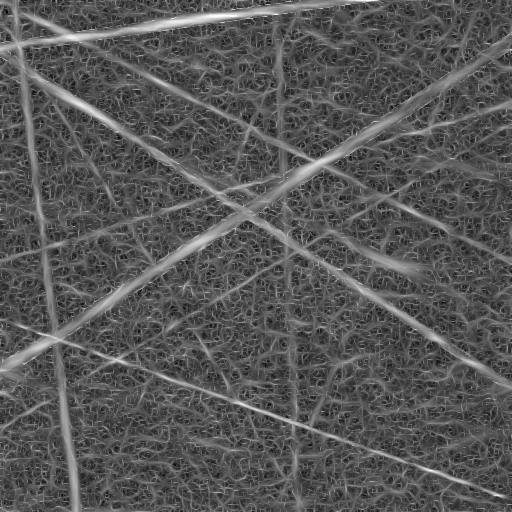
\includegraphics[width=\qtrcol]{\figpath/ipmi/line512_003_lines} &
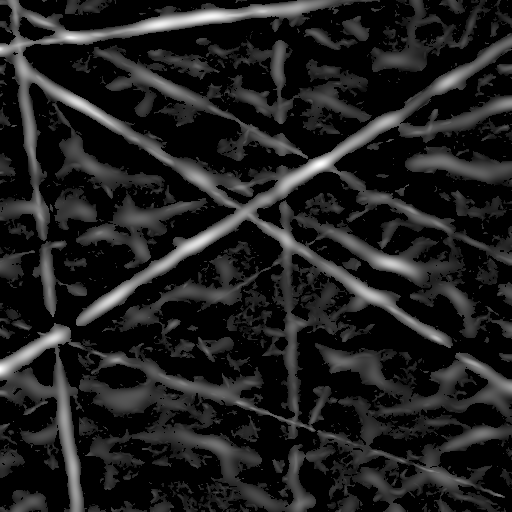
\includegraphics[width=\qtrcol]{\figpath/ipmi/line512_003_gaussian} &
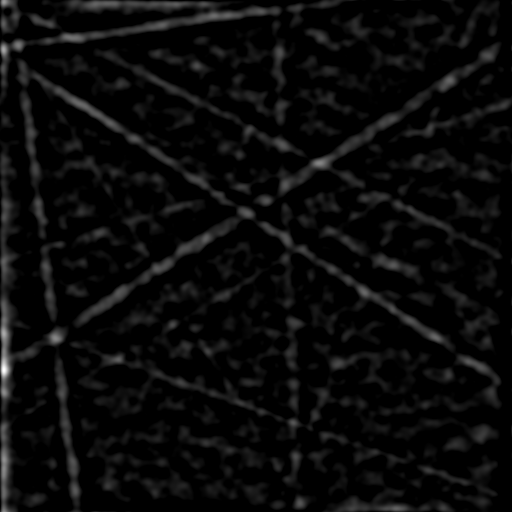
\includegraphics[width=\qtrcol]{\figpath/ipmi/line512_003_monogenic} \\
(a) & (b) & (c) & (d) \\
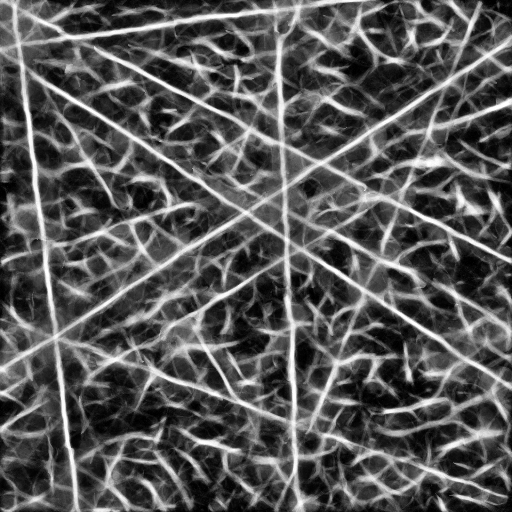
\includegraphics[width=\qtrcol]{\figpath/ipmi/line512_003_rf_191905} &
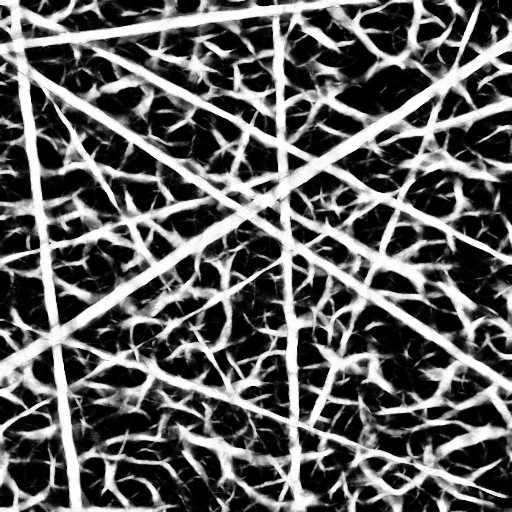
\includegraphics[width=\qtrcol]{\figpath/ipmi/line512_003_rf_191961} &
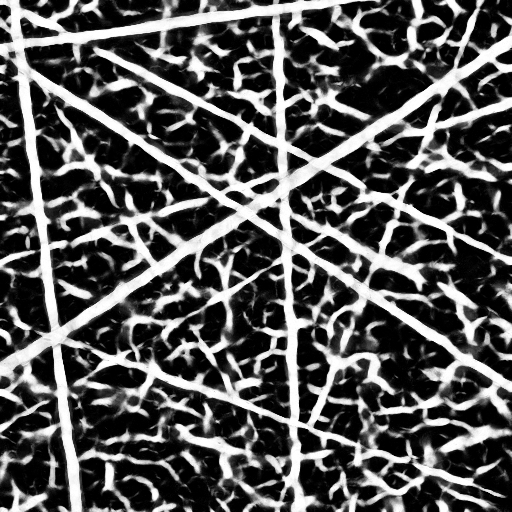
\includegraphics[width=\qtrcol]{\figpath/ipmi/line512_003_rf_233141} &
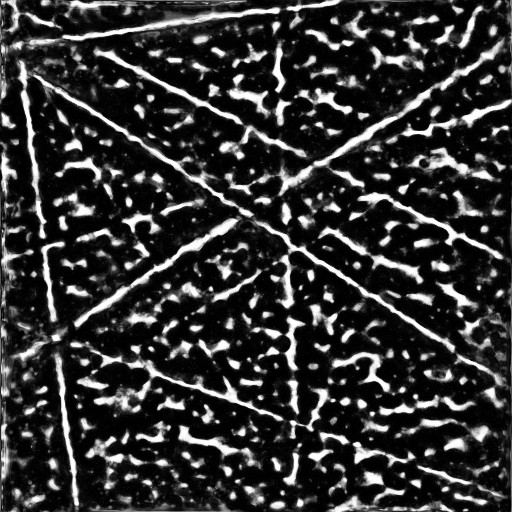
\includegraphics[width=\qtrcol]{\figpath/ipmi/line512_003_rf_191960} \\
(e) & (f) & (g) & (h)
\end{tabular}
%
\caption{Synthetic test image and corresponding filter responses: (a) original image; (b) Linop; (c) Gaussian; (d) Monogenic; (e) DT-CWT/RF; (f) Linop/RF; (g) Gaussian/RF; (h) Monogenic/RF.}
\label{f:synthetic_responses}
\end{figure}


\begin{figure}
\centering
\begin{tabular}{c c c c}
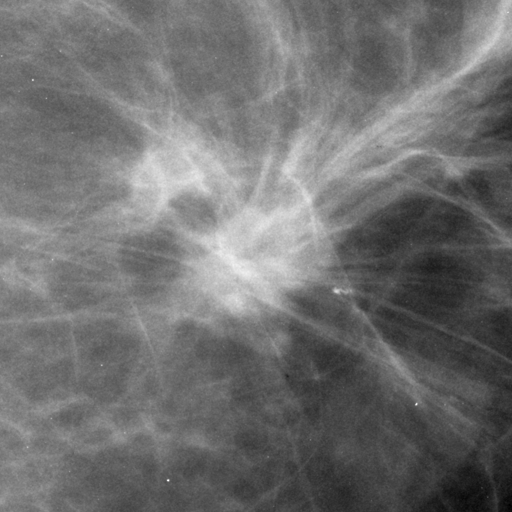
\includegraphics[width=\qtrcol]{\figpath/ipmi/mass028} &
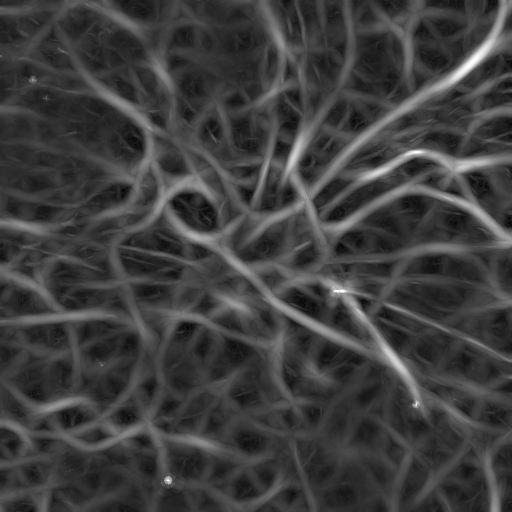
\includegraphics[width=\qtrcol]{\figpath/ipmi/mass028_linop} &
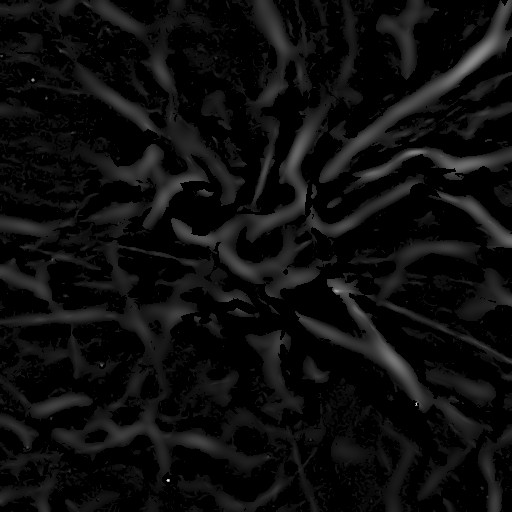
\includegraphics[width=\qtrcol]{\figpath/ipmi/mass028_gaussian} &
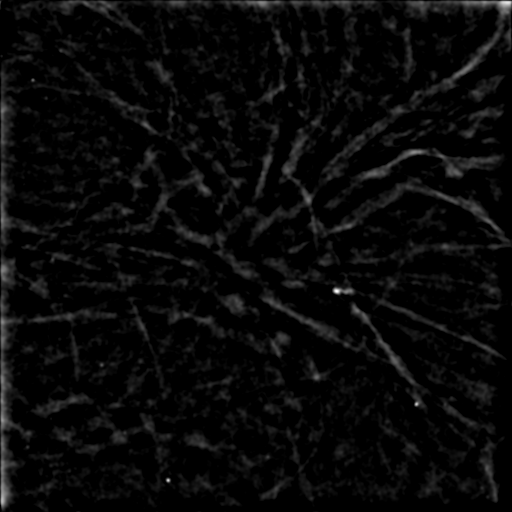
\includegraphics[width=\qtrcol]{\figpath/ipmi/mass028_monogenic} \\
(a) & (b) & (c) & (d) \\
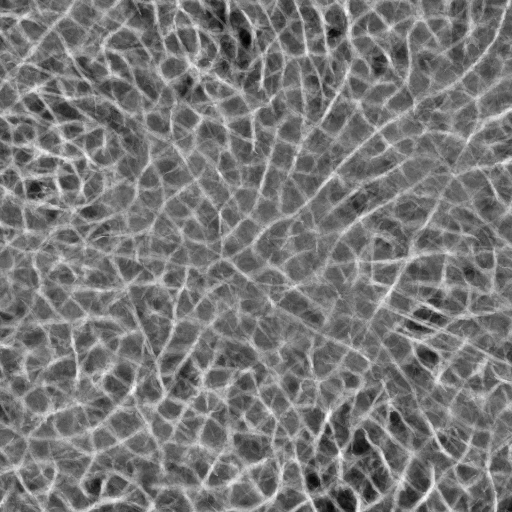
\includegraphics[width=\qtrcol]{\figpath/ipmi/mass028_dt} &
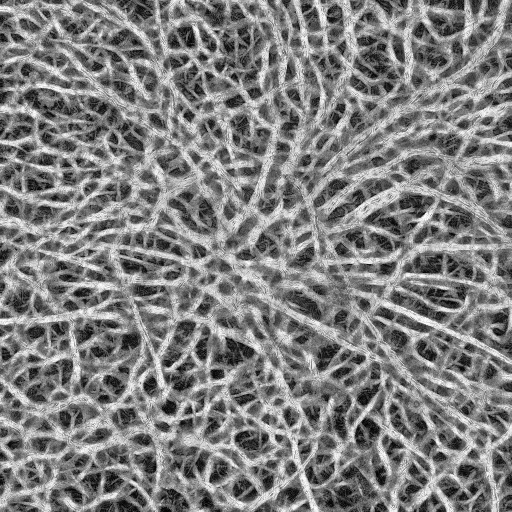
\includegraphics[width=\qtrcol]{\figpath/ipmi/mass028_rf_linop_w1l5} &
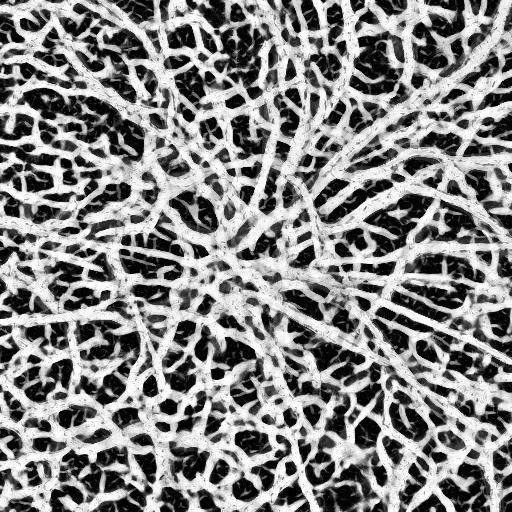
\includegraphics[width=\qtrcol]{\figpath/ipmi/mass028_rf_gaussian} &
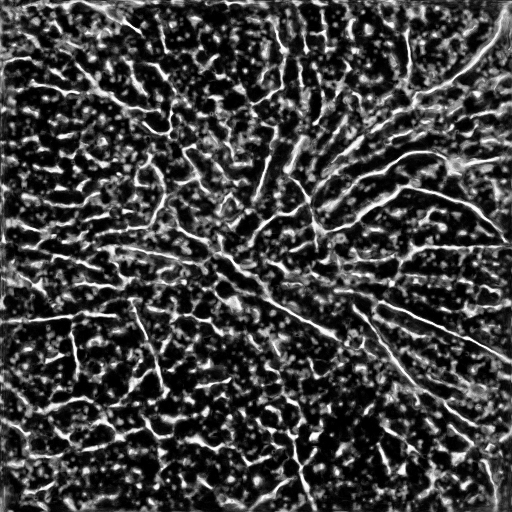
\includegraphics[width=\qtrcol]{\figpath/ipmi/mass028_rf_monogenic_w3l4} \\
(e) & (f) & (g) & (h)
\end{tabular}
%
\caption{Mammogram region containing malignant spiculated mass and corresponding filter responses: (a) original image; (b) Linop; (c) Gaussian; (d) Monogenic; (e) DT-CWT/RF; (f) Linop/RF; (g) Gaussian/RF; (h) Monogenic/RF.}
\label{f:real_responses}
\end{figure}


\begin{figure}
\centering
\begin{tabular}{c c c}
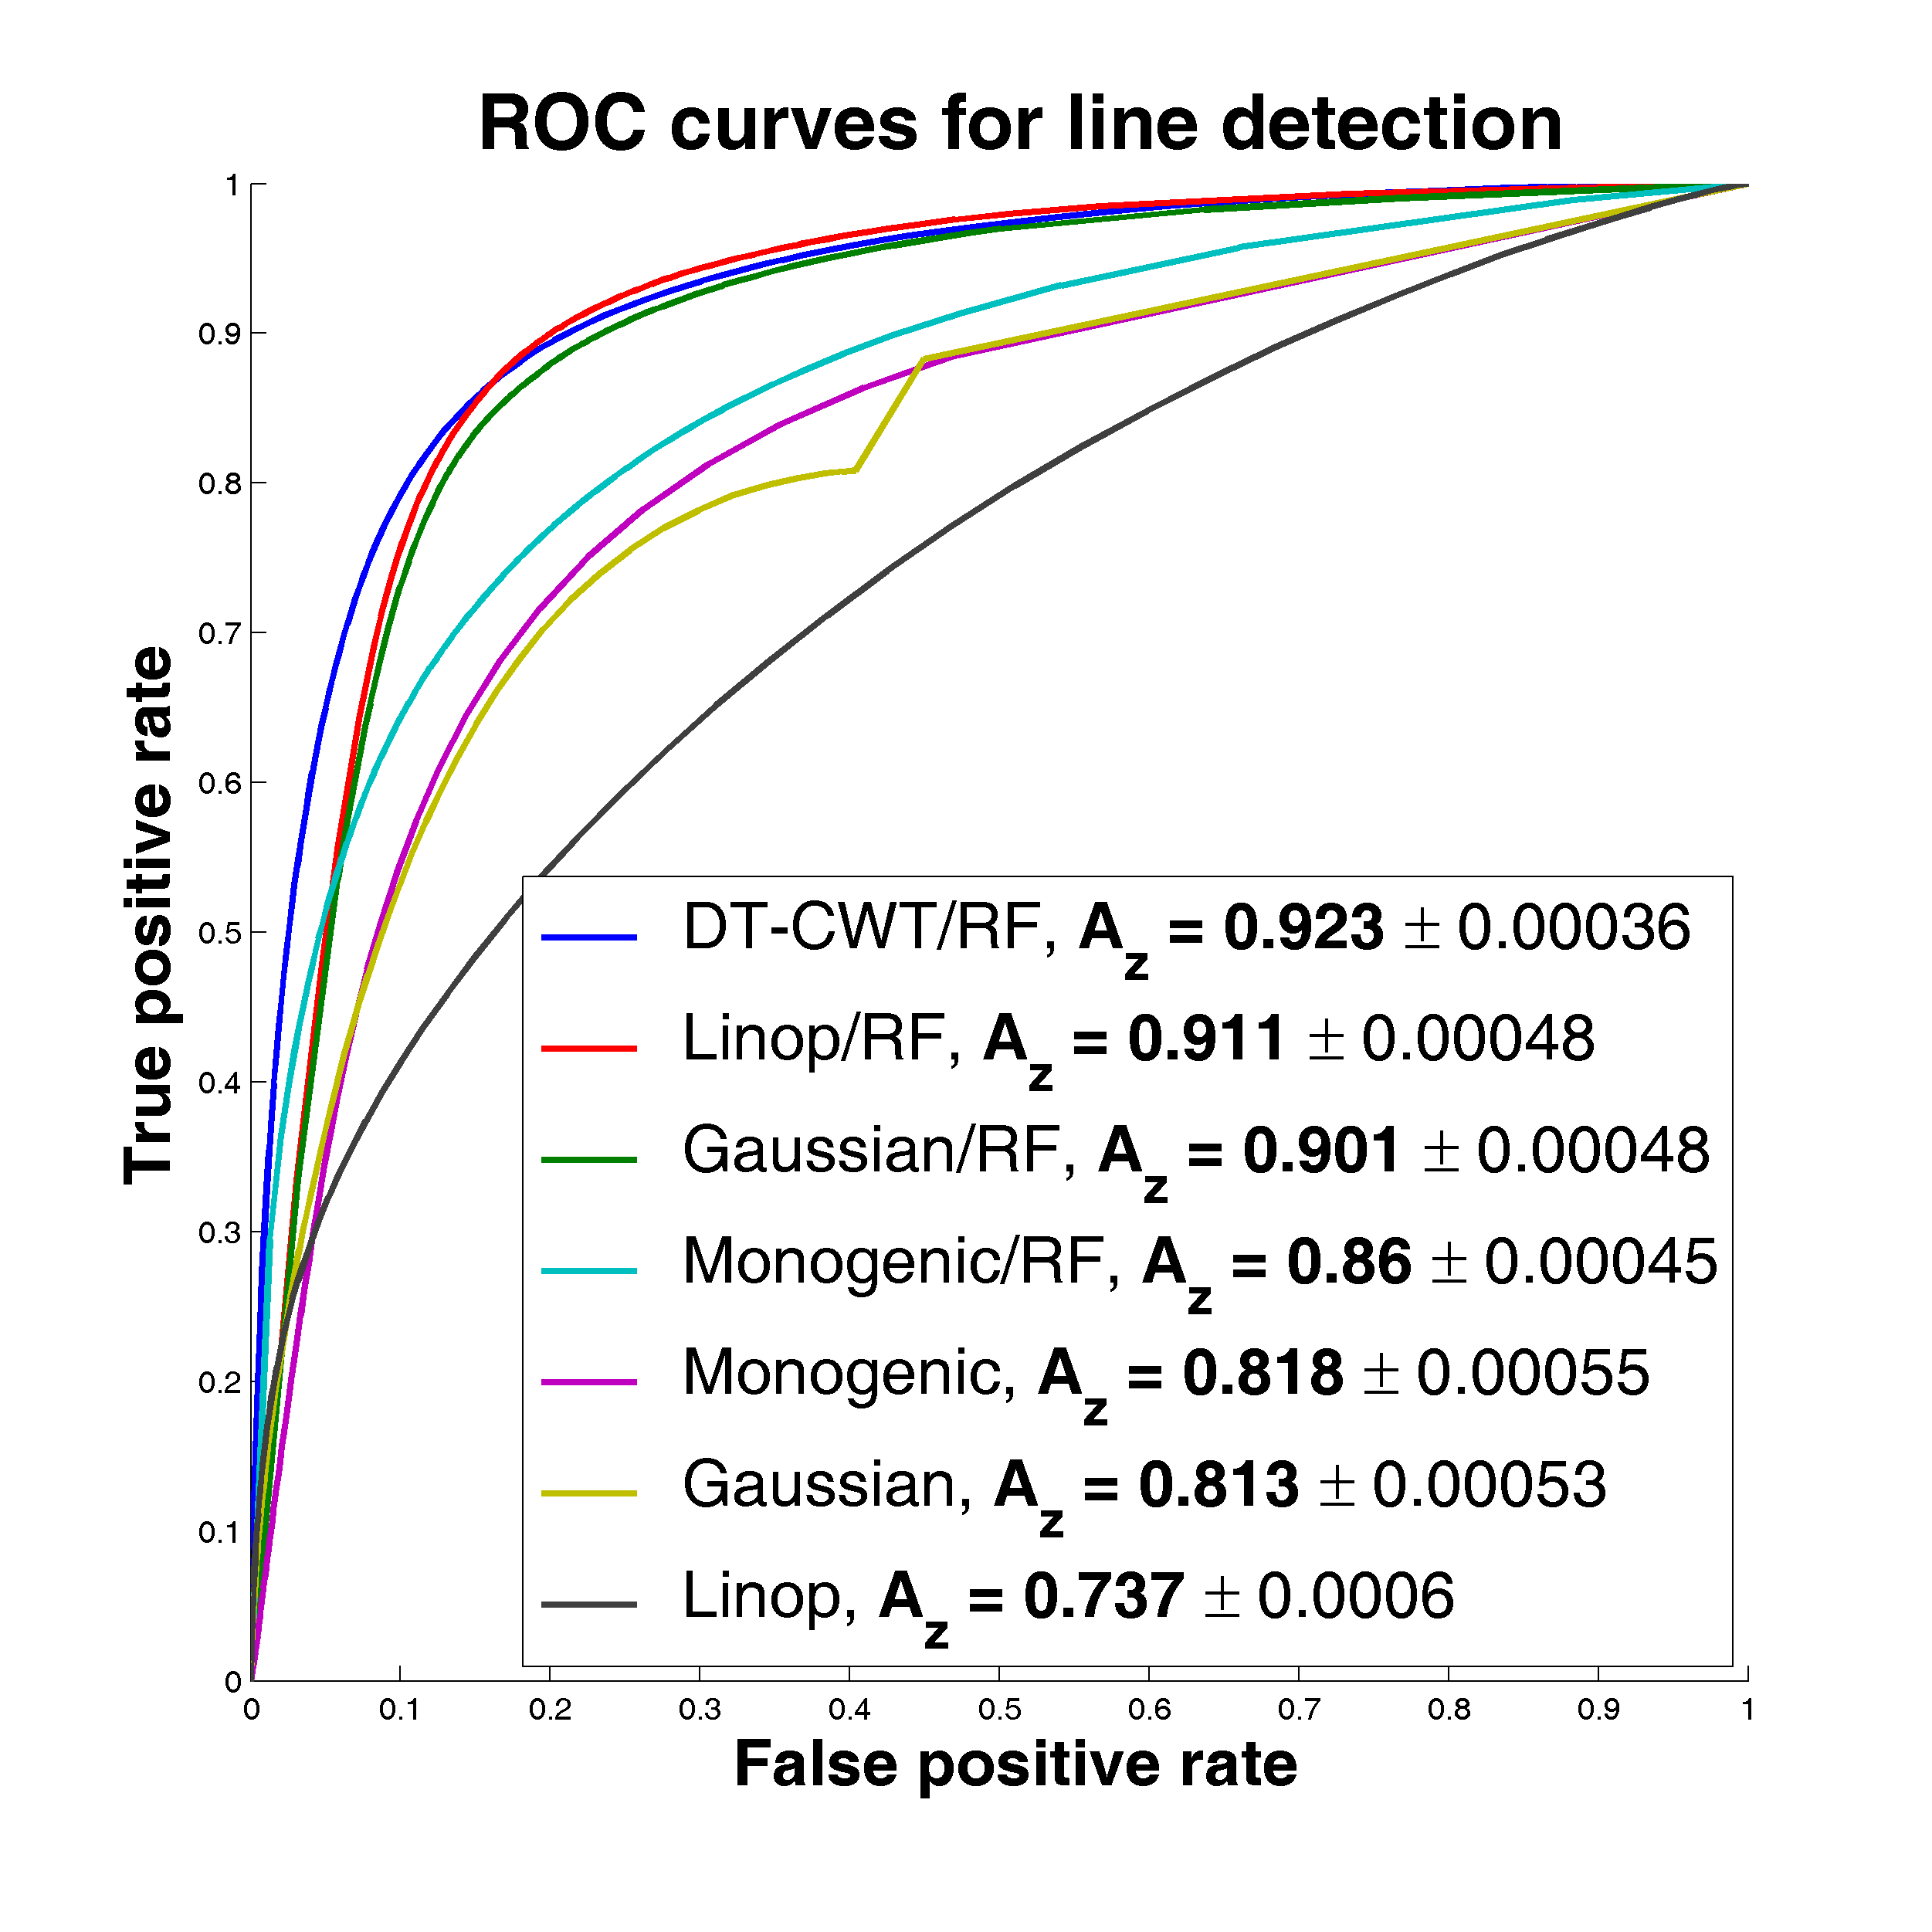
\includegraphics[width=0.33\columnwidth]{\figpath/ipmi/line_detection_roc} &
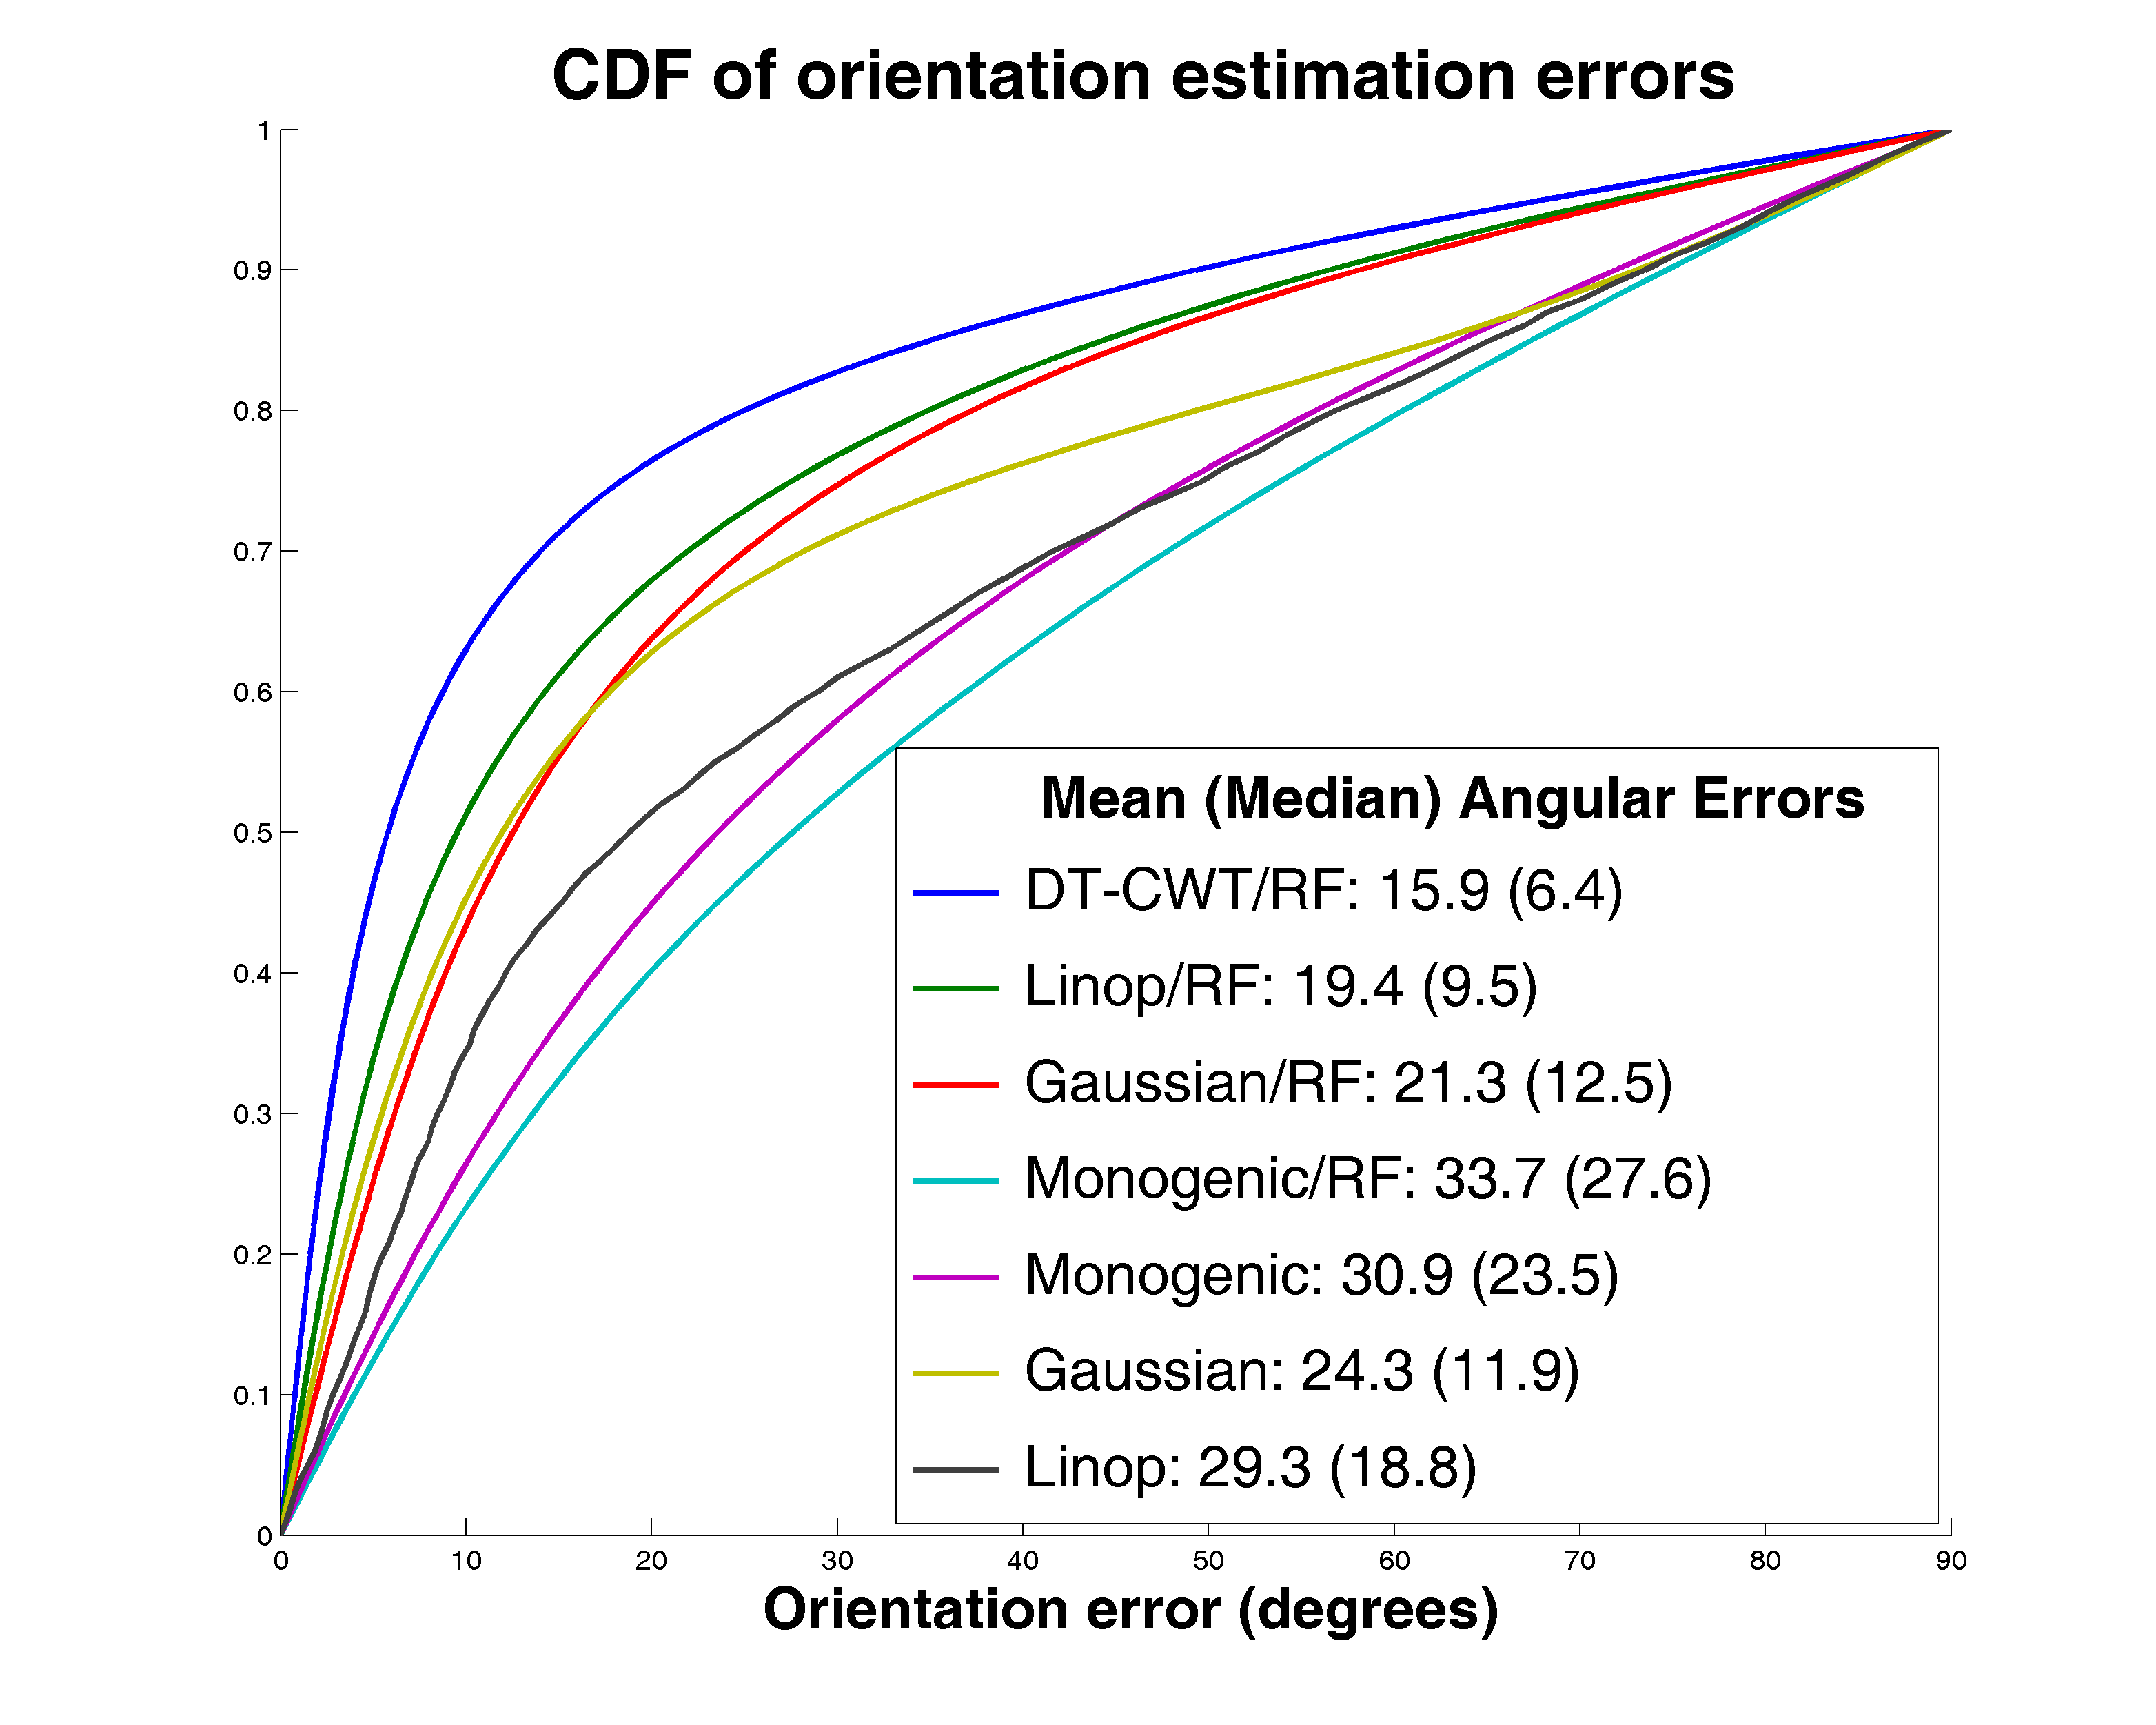
\includegraphics[width=0.33\columnwidth]{\figpath/ipmi/orientation_estimation_cdf} &
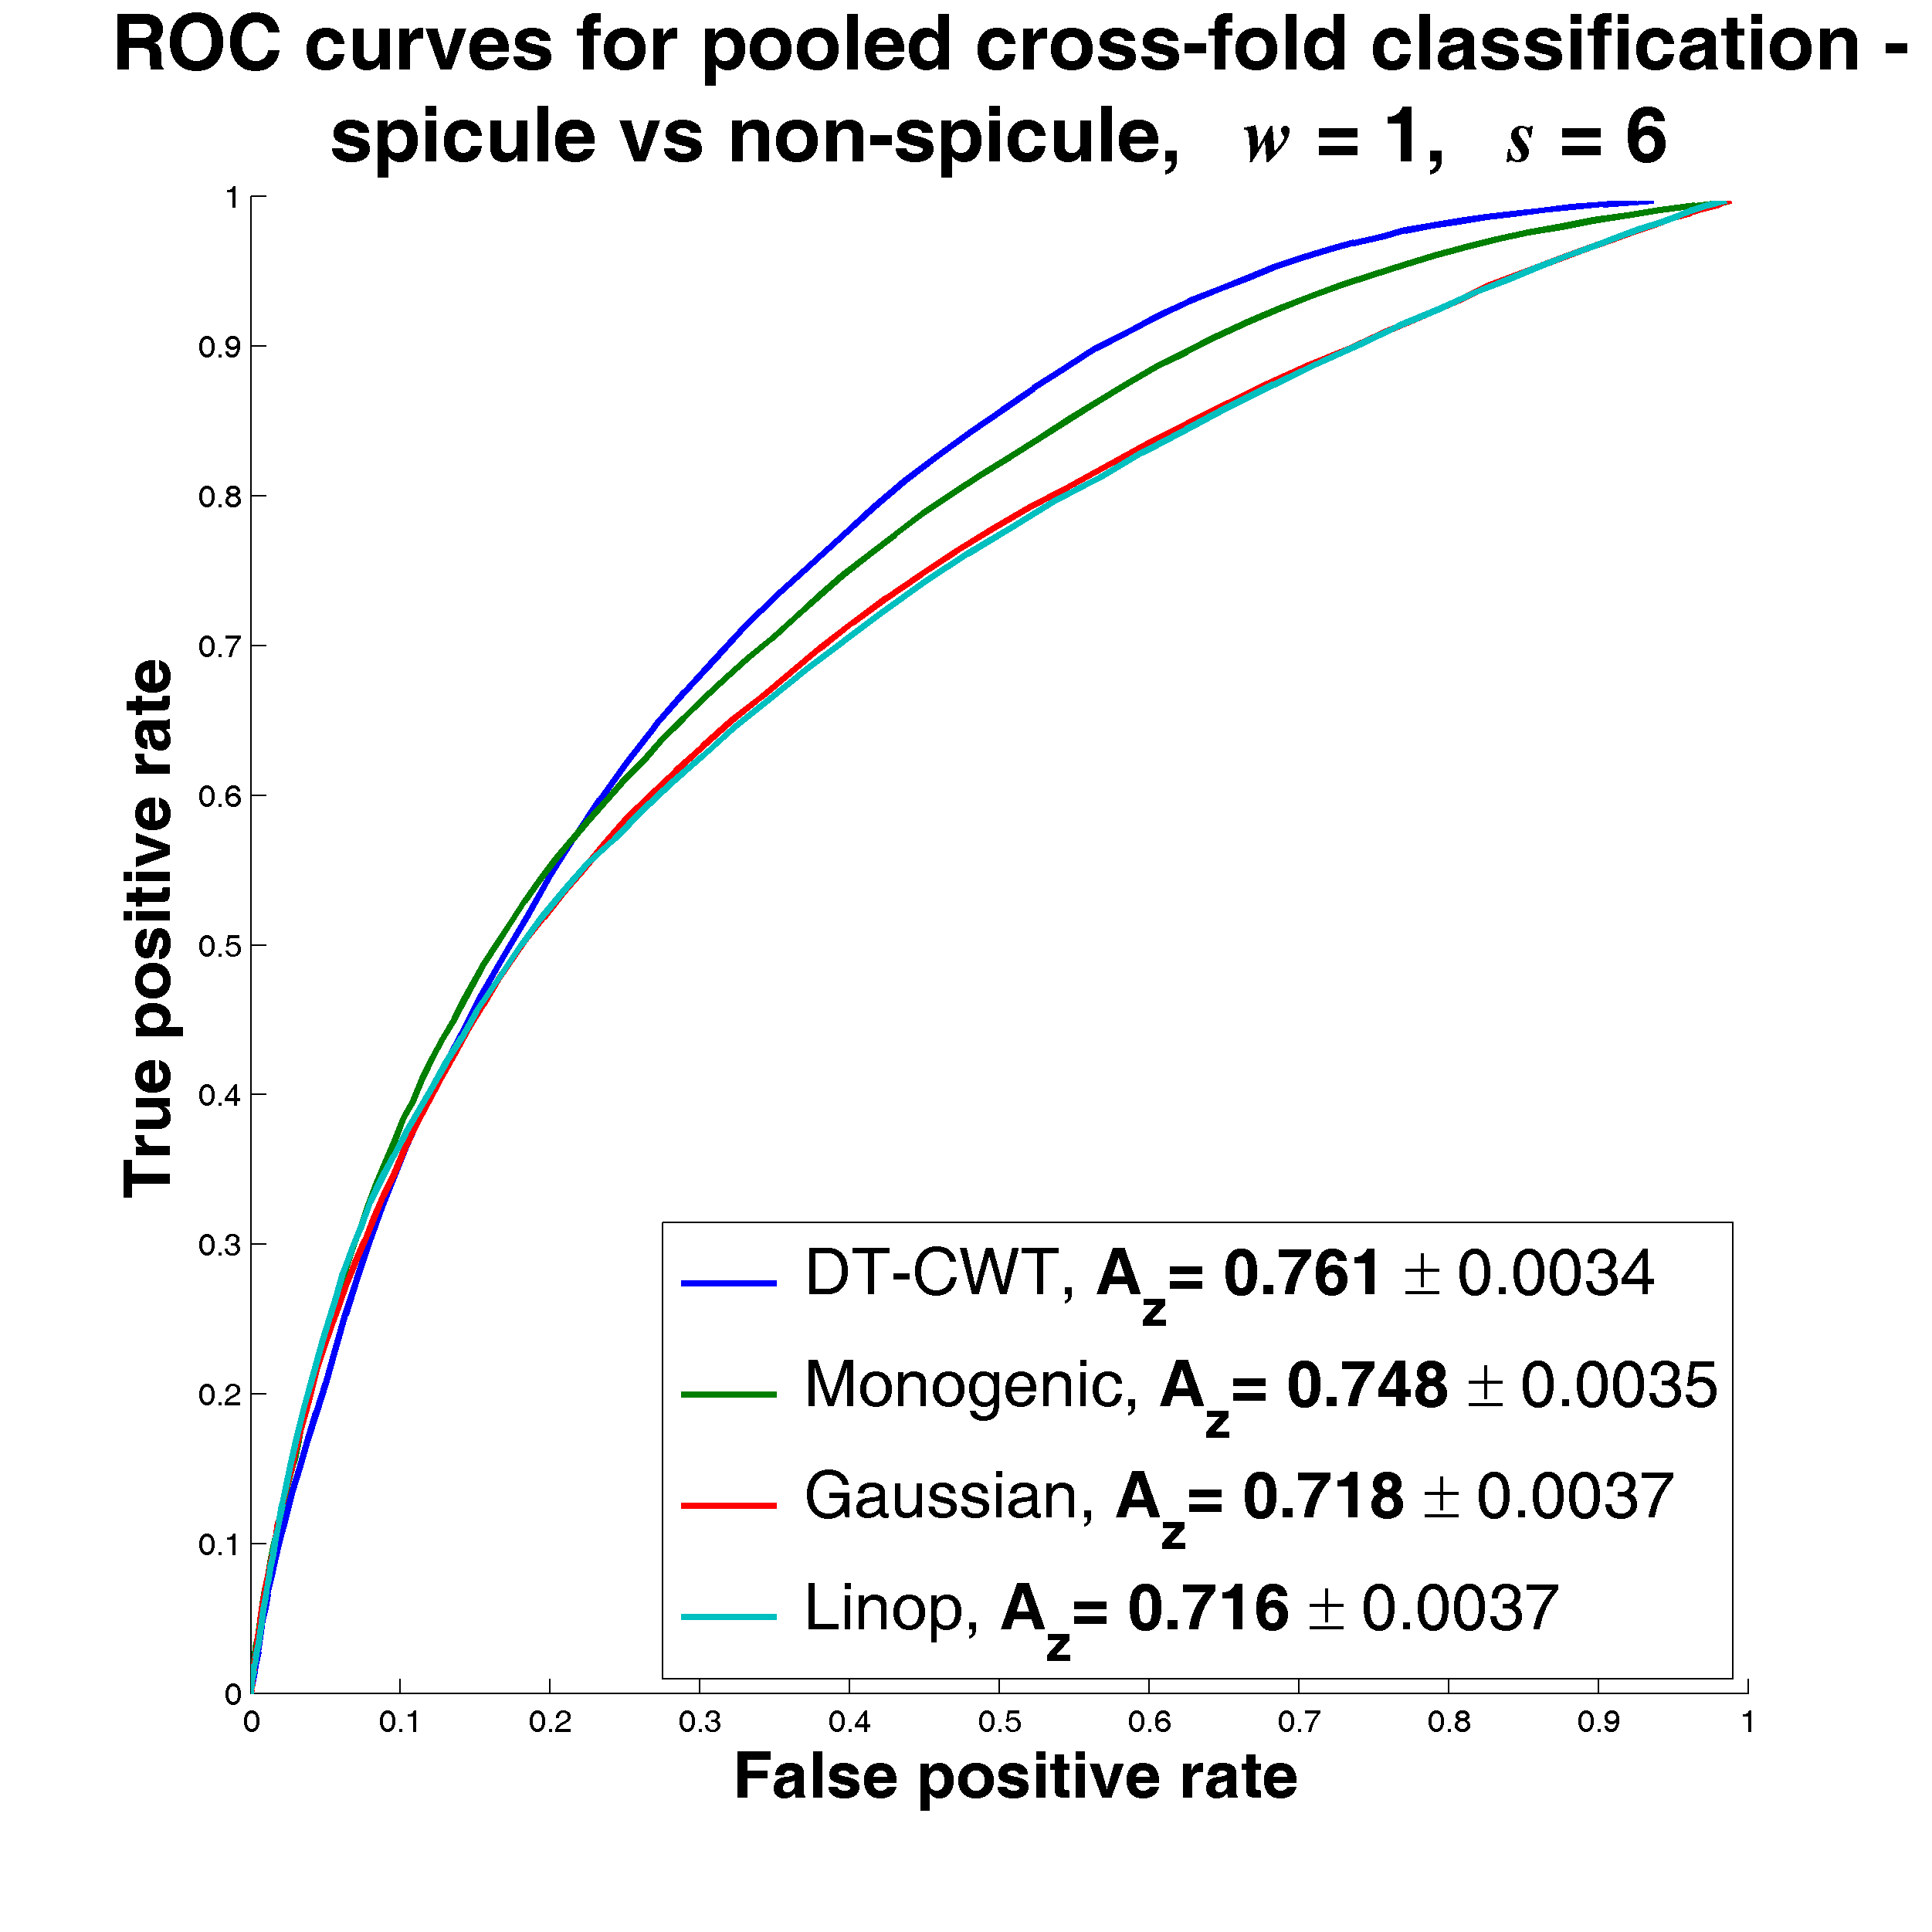
\includegraphics[width=0.33\columnwidth]{\figpath/ipmi/rf_spic_1_6}
\end{tabular}
%
\caption{Receiver operating characteristic (ROC) curves for different curvilinear structure detection methods; centre: Cumulative distribution functions (CDF) of errors in orientation estimation for the different methods; right: ROC curves for spicule classification.}
\label{f:detection_roc}
\end{figure}


\begin{table}
\centering
\caption{Line detection and orientation computation results. For every algorithm, we present the area under the ROC curve ($A_z$), the sensitivity at 90\% specificity, and the mean absolute error of the orientation estimate.}
\label{t:line_detection}
%
\begin{tabular}{l c c c}
Algorithm	
		& $A_z$							& Sens. \@ 90\% spec. & MAE \\
\hline
DT-CWT/RF ($w$ = 1, $s$ = 5)												
		& 0.923$\pm$0.00036	& 0.792 							& 15.88 \\
Linop/RF ($w$ = 1, $s$ = 5, 8 orientations)				
		& 0.911$\pm$0.00048	& 0.757								& 19.35 \\
Gaussian/RF ($w$ = 1, $s$ = 4, $\sigma_{min}$ = 1)
		& 0.901$\pm$0.00048	& 0.731								& 21.37 \\
Monogenic/RF ($w$ = 1, $s$ = 4, $\lambda$ = 4)
		& 0.868$\pm$0.00045	& 0.643								& 33.73 \\
Monogenic ($s$ = 3, $\lambda$ = 4)									
		& 0.818$\pm$0.00055	& 0.547								& 30.86 \\
Gaussian ($s$ = 4, $\sigma_{min}$ = 1)							
		& 0.813$\pm$0.00053	& 0.533								& 24.27 \\
Linop ($s$ = 5, 8 orientations)										
		& 0.737$\pm$0.00060	& 0.413								& 29.32 \\
\end{tabular}
\end{table}


\begin{table}
\caption{Results for spicule classification. For every algorithm, we show the area under the ROC curve ($A_z$)}
\label{t:spicule_classification}
%
\begin{tabular}{l c}
Algorithm
		& ROC $A_z$ \\
\hline
DT-CWT/RF ($w$ = 1, $s$ = 6, all orientations)
		& 0.761$\pm$0.0034 \\
Monogenic/RF ($w$ = 1, $s$ = 5, 8 orientations)
		& 0.748$\pm$0.0035 \\
Gaussian/RF ($w$ = 1, $s$ = 5, $\sigma_{min}$ = 1)
		& 0.718$\pm$0.0037 \\
Linop/RF ($w$ = 1, $s$ = 5, $\lambda$ = 4)
		& 0.716$\pm$0.0037 \\
\end{tabular}
\end{table}
